\documentclass{article}
\usepackage{graphicx} % Required for inserting images
\usepackage[natbibapa]{apacite}
\usepackage[colorlinks=true,linkcolor=black,citecolor=black,urlcolor=black]{hyperref}


\title{\vspace{-2cm}Assignment 1\\
    The Scientific Discourse}

\author{Tymur Mykhalievskyi\\ 7031100}
\date{\today}


\begin{document}

\maketitle

\section{General Overview}
The original work by \cite{reshef2011} introduces a new metric called MIC. The topic quickly gained popularity and was followed by a number of papers that either criticize the work or try to improve it. In this review we will focus on the critique towards MIC. The main goal of this review is to provide a critical overview of the work by \cite{reshef2011} and to discuss the limitations of MIC. 

\section{Scientific Discourse on MIC}
In my opinion, the work by \cite{reshef2011} got a lot of attention because it was the first work that introduced a new metric that is supposed to be general and equitable. But even more importantly, the whole idea of MIC seems rather intuitive, does not involve complicated mathematics and was tested on empirical data. The first critique towards MIC was presented by \cite{simon2014}. The following quote summarizes the main point: 
\begin{quote}
    ``This set of dependencies is by no means exhaustive, however it suggests that MIC has serious power deficiencies, and hence when it is used for large-scale exploratory analysis it will produce too many false positives. The ``equitability'' property of MIC is not very useful, if it has low power.''
\end{quote}

I would agree with the main point of lack of power by \cite{simon2014}. However, due to low power, the metric would be prone to false negatives rather than false positives as authors suggested. That is, the metric would assign too low scores to the noisy relationships and therefore would not be able to detect them. 

Further, more thorough critique by \cite{kinney2014} tries to argue that the metric is not as equitable as it is claimed to be. The main problem is that \cite{reshef2011} did not provide a formal definition of equitability, but rather an operationalization. Hence, \cite{kinney2014} suggested a formal definition of equitability that they call ``self-equitability''. While some of the points were definitely valid, such as inconsistency of MIC \citep{kinney2014} (Figure 3), the main point of the paper is that the metric is not ``self-equitable'' enough, which it never claimed to be. 

\sloppy
Hence, there appeared an expected response by \cite{reshef2014}. They pointed out that ``self-equitability'' was not the goal of the original work. Furthermore, \cite{reshef2014} were not satisfied with the comparisons of MIC and another mutual information estimation method by \cite{kinney2014}. Therefore, a more thorough comparison was made. However, the main problem remains, equitability according to \cite{reshef2014} is still not formal and definitely does not align with self-equitability. 

The follow up by \cite{kinney20142} points out exactly the same problem. Equitability by \cite{reshef2014} is still not defined formally, therefore, allowing \cite{reshef2014} to interpret the results in a way that is convenient for them.

Finally, the formal definition according to \cite{reshef2015} was presented, and similar results to their last response were shown \citep{reshef2014}.

\subsubsection*{Conclusion}
To summarize, the discourse around MIC was justified in my opinion. Every author is biased till some extent, and therefore, seeing different points of view is crucial. 

One could argue that the original work by \cite{reshef2011} should not have been published in the first place, as it does not provide a formal definition of equitability. However, I would argue that the work was important and necessary for science. The metric is definitely not perfect, but it is a good starting point for further research. 

PNAS is high-profile and benefits from buzzworthy articles. MIC was such a paper. That said, academic journals do not make money like newspapers, and PNAS is run by the National Academy of Sciences. Therefore, it's unlikely that money alone drove the decision of publishing the comments by \cite{simon2014} and \cite{kinney2014}. 

\section{MIC}
In this section we will critically discuss MIC. The overall idea seems promising on the first glance. MIC is supposed to be the one metric that is general and equitable (according to the definition by \cite{reshef2011}). Reading the work by \cite{reshef2011}, prima facie, MIC completely satisfies these properties. In particular, MIC does not make any assumptions about the underlying function which is supposed to make it generalize very well. However, after reading the concerns presented by \cite{simon2014} and \cite{kinney2014}, a more thorough analysis of MIC had to be conducted.

\subsection{Limitations of MIC}

\subsubsection{Grid Resolution and Time Complexity Trade-Off}
In my opinion, the main problem of MIC lies in the time complexity of the algorithm. Increase in grid resolution leads to an increase in power \citep{cao2021} (Figure 4). On the other hand, the time complexity of the algorithm might be naively estimated by \autoref{eq:1}.

\begin{equation}
    O(n^{1+\alpha}\cdot \log{n})
    \label{eq:1}
\end{equation}

The time complexity is estimated as follows: $B(n) = n^\alpha < xy$ bin combinations are generated, where for each bin combination the algorithm needs to estimate the actual bins. Here, it becomes difficult to estimate the time complexity of the algorithm as the original work by \cite{reshef2011} does not provide any information on the time complexity of the algorithm, even though they mention using a dynamic programming approach. Hence, theoretical time complexity of the dp would be around $O(n\log{n})$ considering that \cite{reshef2011} don not try all possible bin assignments. However, in practice the algorithm runtime is way better estimated by \autoref{eq:2}, which also aligns with tests done by \cite{cao2021} (Table 3).
\begin{equation}
    O(n^{2+\alpha})
    \label{eq:2}
\end{equation}
, aligns with tests done by \cite{cao2021}. Suggesting that either dp is not as efficient as one can assume, or the limit $xy < B(n)$ is not held. Either way, this is not good news for MIC as the metric is only runnable on sets of at most 10000 observations depending on how long one would like to wait. This also means that increasing the resolution of the grid which improves power \citep{cao2021} means an increase in running time which is already rather high.


\subsubsection{Geometrical Interpretation of MIC}
The underlying implementation of MIC is based on the idea of partitioning the scatter plot of two variables into a grid. At this point we can see an important limitation of MIC which also does not align with the equitability of the metric. Due to the fact that the grid is made of rectangles, the relationship some relationships between two variables could work particularly well. For example, if the underlying function is a step function, the grid would capture the relationship very well. However, if we exchange the underlying function to a modular function, the grid would not be able to capture the relationship as well. This is because the step function would be able to fit into the grid cells very well, while the modular function being not parallel to any of the axis would not be able to fit into the grid cells. This particular case is visualized in \autoref{fig:step_mod}. Notice that the step function is assigned with MIC score of 1, while the modular function only achieves a score around 0.7. It is worth noting that by no means a thorough comparison is made here. This is only a demonstration of a particular case. However, the effect persists for other values of the parameters. The reason for this is only in the fact that the grid is made of rectangles. Therefore, a more rectangular and parallel to the axis function would be able to fit into the grid cells better. Therefore, getting a higher MIC score.

\begin{figure}
    \centering
    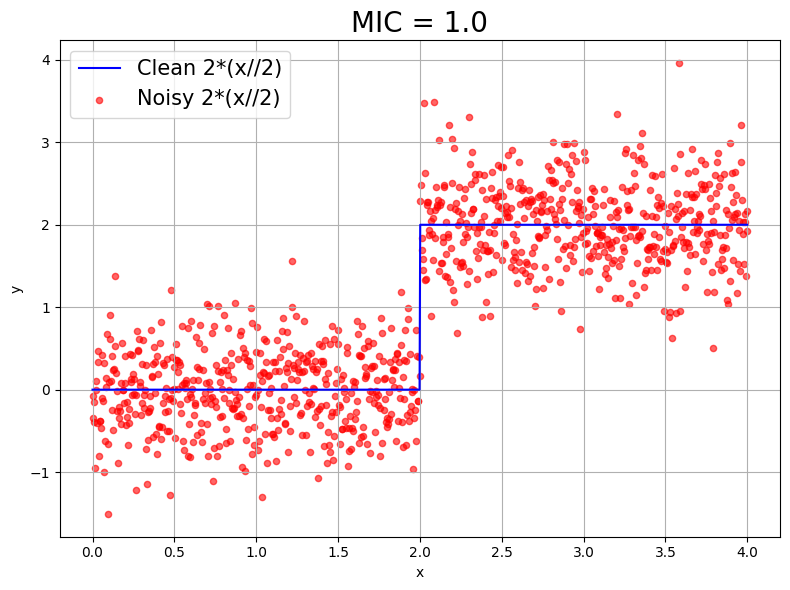
\includegraphics[width=0.47\textwidth]{images/step1.png}
    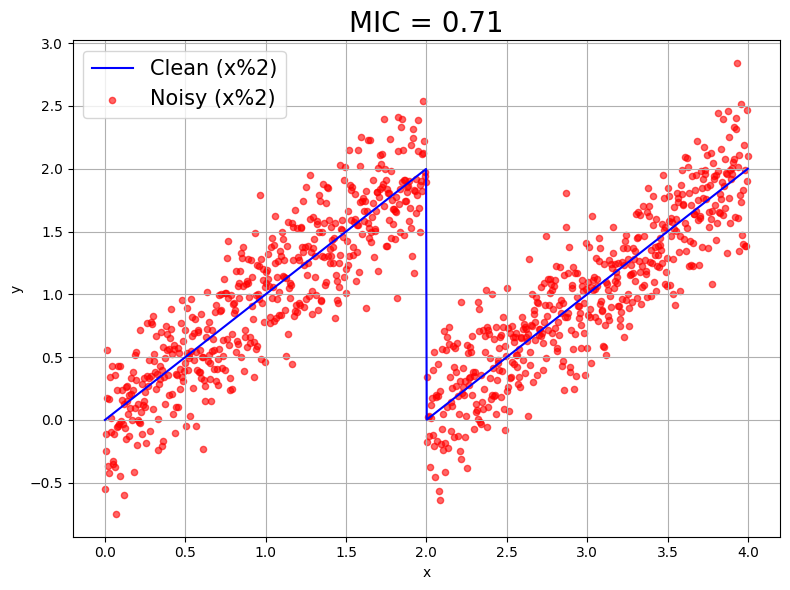
\includegraphics[width=0.47\textwidth]{images/mod1.png}
    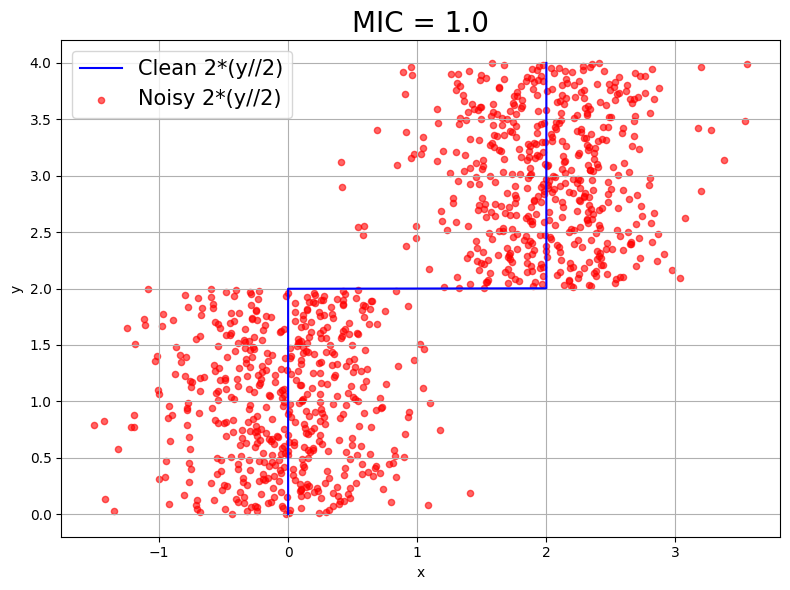
\includegraphics[width=0.47\textwidth]{images/step2.png}
    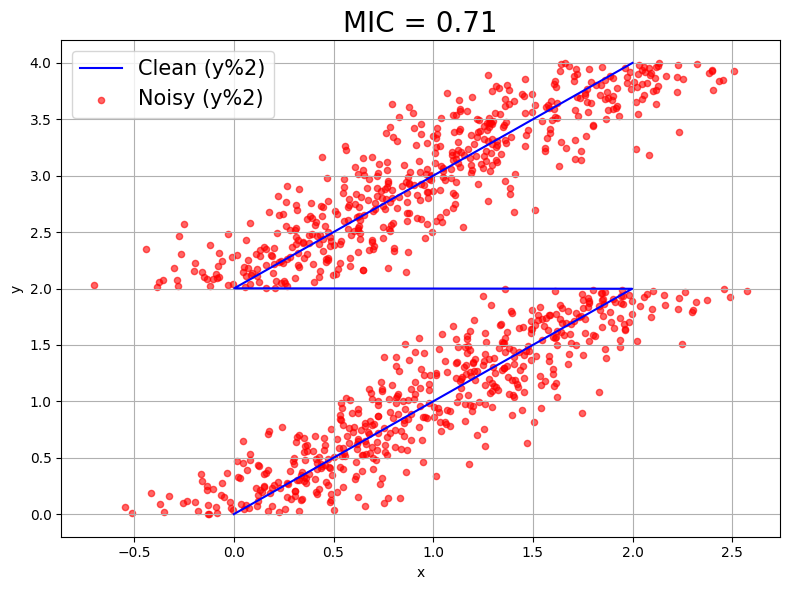
\includegraphics[width=0.47\textwidth]{images/mod2.png}
    \caption{Comparison of the step function and modular function. The left plot shows the step function with its inverse variant on the bottom. While the right plot shows the modular function with its inverse variant. Both plots were generated using the exact same parameters: $n = 1000, 1-R^2=0.2, x\in [0, 4)$. The source code is available via GitHub under ``Assignment 1'' \citep{src}.}
    \label{fig:step_mod}
\end{figure}

\section{Equitability}

If one imagines a task, where one is interested in finding any patterns in the data, equitability is a very useful property. As we would want the patterns to be sorted from less noisy to more noisy ones, regards of the actual relationship. An equitable approach would achieve exactly that. Therefore, the equitability is a useful but not sufficient property. The statistical power is also very important, as low statistical power would mean that only the relationships with little noise would be found.


\section{Conclusion}
While MIC is a very interesting metric, it has two issues: low power and high time complexity. That being said MIC might be on a more intuitive level than other mutual information estimators, which could enhance the interpretability. However, currently there is no straightforward way to visualize the best grid as \cite{reshef2011} did (Figure 1). \cite{cao2021} achieved some progress in this task. 



\bibliographystyle{apacite}	
\bibliography{references}


\end{document}


